\refstepcounter{section}
\section*{Lecture 03: From Classical to Quantum}
\addcontentsline{toc}{section}{Lecture 03: From Classical to Quantum }
Inspecting the transition from a classical to quantum description is necessary for understanding QFT, which is just a \textit{sophisticated mechanics}. \\[0.2cm]
We know that the position $q$ and momentum $p$ uniquely define the state of a \textit{classical} particle. $$(q,p)\in \Pi \ \text{(phase space) }\qquad q,p\in \re$$
The Hamiltonian is just a way of doing time evolution. Using the Hamiltonian, we can `fibrate' the phase space, that is, starting from one point, we can go to some other point. Also, note that changing the parameters in the Hamiltonian (eg. $\omega$ in SHO Hamiltonian), we change the fibration patterns. 


\tikzset{every picture/.style={line width=0.75pt}} %set default line width to 0.75pt        

\begin{center}
    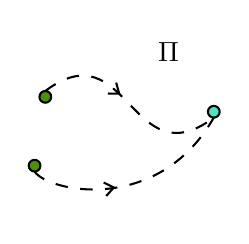
\begin{tikzpicture}[x=0.75pt,y=0.75pt,yscale=-1,xscale=1]
%uncomment if require: \path (0,190); %set diagram left start at 0, and has height of 190

%Shape: Circle [id:dp9514469203911451] 
\draw  [fill={rgb, 255:red, 79; green, 143; blue, 6 }  ,fill opacity=1 ] (144.35,113.82) .. controls (144.35,112.26) and (145.61,111) .. (147.18,111) .. controls (148.74,111) and (150,112.26) .. (150,113.82) .. controls (150,115.39) and (148.74,116.65) .. (147.18,116.65) .. controls (145.61,116.65) and (144.35,115.39) .. (144.35,113.82) -- cycle ;
%Shape: Circle [id:dp6749467169528727] 
\draw  [fill={rgb, 255:red, 79; green, 143; blue, 6 }  ,fill opacity=1 ] (139.18,147) .. controls (139.18,145.44) and (140.44,144.18) .. (142,144.18) .. controls (143.56,144.18) and (144.82,145.44) .. (144.82,147) .. controls (144.82,148.56) and (143.56,149.82) .. (142,149.82) .. controls (140.44,149.82) and (139.18,148.56) .. (139.18,147) -- cycle ;
%Shape: Circle [id:dp598404214978788] 
\draw  [fill={rgb, 255:red, 80; green, 227; blue, 194 }  ,fill opacity=1 ] (225.53,121) .. controls (225.53,119.44) and (226.79,118.18) .. (228.35,118.18) .. controls (229.91,118.18) and (231.18,119.44) .. (231.18,121) .. controls (231.18,122.56) and (229.91,123.82) .. (228.35,123.82) .. controls (226.79,123.82) and (225.53,122.56) .. (225.53,121) -- cycle ;
%Curve Lines [id:da5887758576826126] 
\draw  [dash pattern={on 4.5pt off 4.5pt}]  (147.18,111) .. controls (187.18,81) and (188.35,153.82) .. (228.35,123.82) ;
%Curve Lines [id:da5100878878183484] 
\draw  [dash pattern={on 4.5pt off 4.5pt}]  (142,149.82) .. controls (148.68,159.65) and (201.68,170.65) .. (228.35,123.82) ;
\draw   (181.31,106.98) -- (182.78,112.26) -- (177.3,112.23) ;
\draw   (175.28,155.09) -- (180.19,157.52) -- (176.52,161.59) ;

% Text Node
\draw (200,86.4) node [anchor=north west][inner sep=0.75pt]    {$\mathrm{\Pi}$};


\end{tikzpicture}
\end{center}
In the quantum world, the phase space changes to the Hilbert space $\SH$ while a point in the phase space $(q,p)$ changes to a vector $\ket{\psi}$ in the Hilbert space.\\[0.2cm]
Also, these real variables become Hermitian (self-adjoint) operators \footnote{A self-adjoint operator $\SO$ is such that $\SO = \SO^\dagger$ in all respect, that is, $\SO$ and $\SO^\dagger$ have the same domain and action. In general, $\mathbb{D}(\SO)\subseteq \mathbb{D}(\SO^\dagger)$ where $\mathbb{D}(\cdot)$ represents the domain of some operator. If the domains are not equal but action is same on a restricted domain (mainly occurs in infinite-dimensional spaces), then those operators are not self-adjoint but called \textit{symmetric/Hermitian} (in some places Hermiticity also requires a symmetric operator to be bounded ). }and the classical Poisson bracket now transforms to the commutator.
\begin{align*}
    \text{CM:}&\qquad \{q,p\}=1\\
     \text{QM:}&\qquad [\hat{q},\hat{p}]=i
\end{align*} 
\subsection{Time Evolution}
% \addcontentsline{toc}{subsection}{Time Evolution}
From classical Hamilton's equations of motion, we have:
\begin{alignat*}{3}
    \dot{q} &= \{q,H\} &&= \pdv{H}{p}  \\
    \dot{p} &= \{p,H\} &&= -\pdv{H}{q}
\end{alignat*}
If $z = \mqty(p\\q)$ is a $2n$ dimensional vector, then $\dot{z} = \{z,H\}$. Now, in quantum we know:
$$i\hbar \pdv{\ket{\psi}}{dt} = H\ket{\psi}$$
In both classical and quantum case, the time derivative of a quantity is equal to some action of the Hamiltonian on that quantity (classical \rightarrow \ Poisson bracket, quantum \rightarrow \ Multiplication with Hamiltonian)\footnote{A better analogy would be to use density matrices which gives the von Neumann equation which uses commutator bracket}. \\[0.2cm]
The Hamiltonian in position basis becomes: $$H = \frac{-\hbar^2}{2m}\grad^2 + V$$
And the energy and momentum operators become $E\rightarrow i\hbar \pdv{t}$ and $p\rightarrow -i\hbar \grad$.
\subsubsection{Free Particle}
% \addcontentsline{toc}{subsubsection}{Free Particle}
The dispersion relation for a non-relativistic free particle is:
$$E = \frac{p^2}{2m}$$
The typical solution can be written as $e^{i(\vb{k}\cdot\vb{x}-\omega t)} = e^{\frac{i}{\hbar}(\vb{p}\cdot\vb{x} - Et)} \equiv \exp(-\frac{i}{\hbar}p^\mu x_\mu)$ where we have used the index repeated summation notation and taken the $(+,-,-,-)$ convention.\\[0.2cm]
For a relativistic free particle, the dispersion relation becomes:
$$E^2 = mc^4 + p^2c^2$$
Substituting the energy and momentum operators here, we get:
\begin{alignat*}{3}
    &\qquad\qquad(i\hbar)^2 \pdv[2]{\psi}{t} &&= (-i\hbar)^2c^2 \grad^2\psi + m^2c^4\psi\\
  \implies  & \hbar^2 \pdv[2]{\psi}{t} - \hbar^2c^2\grad^2\psi &&= -m^2c^4\psi\\
  \implies & \quad \frac{1}{c^2} \pdv[2]{\psi}{t} -\grad^2\psi &&= \frac{-m^2c^2}{\hbar^2}\psi
\end{alignat*}
The above equation is called the \textit{Klein-Gordon equation}. In covariant notation, we can compactly write it as:
$$\qty(\partial_\mu \partial^\mu +\qty(\frac{mc}{h})^2)\psi = 0$$
\subsubsection{Continuity Equation}
% \addcontentsline{toc}{subsubsection}{Continuity Equation}
Taking the complex cojungate of the Schr\"odinger's equation and then after some algebraic manipulation, we obtain:
\begin{align*}
     \pdv{(\psi^*\psi)}{t} = \frac{i\hbar}{2m} \grad \cdot \qty[\psi^*(\grad\psi) - \psi (\grad \psi^*)]
\end{align*}
Here, we identify:
$$\rho := \psi^*\psi\qquad\qquad \vb{J} = \frac{-i\hbar}{2m}\qty[\psi^*(\grad\psi) - \psi (\grad \psi^*)]$$ which yields the well-known form of the \textit{continuity equation}:
$$\pdv{\rho}{t} + \grad\cdot\vb{J} = 0$$
Note that in this case, $\rho$ is a positive-definite quantity and can indeed have the interpretation of probability. Also, note that if $\psi$ somehow becomes real-valued, then $\vb{J}=0$ which implies that $\rho$ is constant in time (though it can change in space). \\[0.2cm]
Doing the same thing to Klein-Gordon equation yields:
$$\frac{1}{c^2}\pdv{t}\qty(\psi^*\pdv{\psi}{t}-\psi\pdv{\psi^*}{t})-\grad\cdot\qty(\psi^*\grad{\psi}-\psi\grad{\psi^*})=0$$
From this equation, we can identify:
$$\rho :=  \qty(\psi^*\pdv{\psi}{t}-\psi\pdv{\psi^*}{t}) \qquad\qquad \vb{J} := - c^2\qty(\psi^*\grad{\psi}-\psi\grad{\psi^*})$$
Note the apparent problems with this identification:
\begin{itemize}
    \item It is not apriori obvious that $\rho$ is positive-definite and hence has problem with probability interpretation.
    \item The equation is second-order in time and hence $\rho$ seems to have a term evolving forward and one term evolving backward in time. 
    \item The dispersion relation does not have a single solution; the solutions are $\pm E$
\end{itemize}
The thing is, KG equation treats time and space on equal footing (unlike Schr\"odinger equation where time was in first order and space was in second order). Hence we have to consider all possibilities of moving back and forth in both space and time. 